\documentclass{report}
\usepackage{multirow}
\usepackage{graphicx}
\usepackage{amsmath}
\usepackage{wrapfig}
\usepackage[backend = biber]{biblatex}
\usepackage[utf8]{inputenc}
\addbibresource{references.bib}

\title{CS 251 Project Report \\ Fire Extinguisher \\ Group 30 - Hackstreet Boys}
\author{Sanat Anand - 140040005 \\ Siddhant Garg - 14D070027 \\ Ritwick Chaudhry - 14D070063}
\date{October 2015}

\begin{document}

\maketitle

\tableofcontents
\pagebreak

\chapter{Original Project Idea}
\section{Aim of the project}
This project aims to create a simulation of a Rube-Goldberg machine which extinguishes a fire using the Box2d physics engine for C++.

\section{Motivation}
While browsing through lots of ideas of Rube Goldberg machines \cite{Rube-Goldberg} we felt that we should make something that will not just be a simulation made from balls and blocks but something more. As a result we came up with the idea of taking inspiration from how a dam produces electricity. In a dam, water gets released from height and falls on the blades of a turbine which causes it to rotate and thus produce electricity \cite{Hydro-pump}. Since we were to include at least 10 moving components, so we decided to extrapolate on this idea. We were also quite impressed by the Rube Goldberg machine ideas using balloons and decided to also include one such element. We wanted the whole machine to end with something productive and thus we put the idea of extinguishing a fire with water.\cite{Extinguisher}\\

\section{Plan}
The Rube Goldberg simulation starts off with water falling off a dam. Here we will be using small droplets of water instead of using a continuous vessel full of water. As a result, the water droplets will fall down through the pipe and will hit the blades of the turbines. This will result in the turbine rotating and thereby making the above pulley rotate along with it (as both of them are joined by a belt). This rotating of the above pulley will extend the rope and cause the horizontal plank to go down. As a result, the horizontal plank falls down and pushes into the air-pump. This causes the balloon attached to the pump getting filled and starting to rise. As the balloon rises, it pushes one side of the see-saw thereby causing the ball resting on the see-saw to fall onto the set of planks. As the ball falls down and moves to the right of the plank, it pushes the vertical plank which causes the plank to in turn push the ball present on the lower plank. This continues till the last ball finally drops and leaves the plank. This ball then pushes the glass full of water which causes the fire to get extinguished.\\

\section{Diagram}
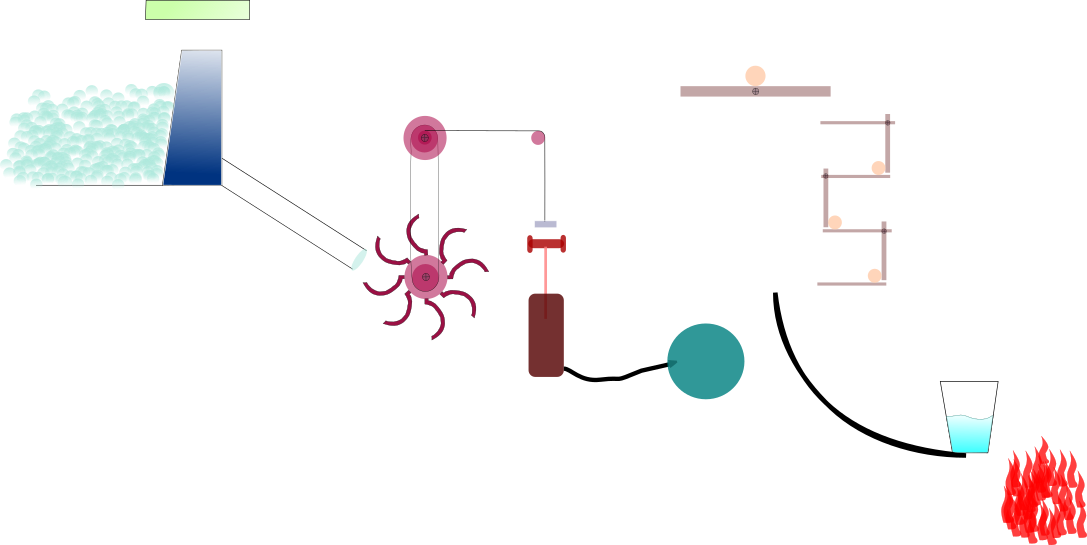
\includegraphics[scale=0.4]{grp_30}\\

\chapter{Final Project}
\section{Design Changes}
Our original idea of using a dam mechanism to extinguish fire remains unchanged. We have implemented everything we had proposed with minor changes. In addition we have also incorporated lots of additional features and have greatly enhanced the complexity of the machine in order to make the whole simulation more interesting. 

\subsection{Major Features}
The most important feature is a \textbf{Water conservation model} wherein the water which is dispatched from the dam is fed back to it. To achieve this, water is collected in a tub after passing through the turbine and this tub is lifted to the dam through an elevator shaft. Through this, close to ~90\% water is saved and returns to the dam. In order to trigger the mechanism, we have used the balloon (from the main mechanism) which hits a shaft and releases a ball. This ball then hits a series of dominoes. The last domino hits another ball which falls and moves to hit a shaft which pushes the tub filled with water towards the left. The whole simulation is synchronised such that when the tub reaches the end of the plank, an elevator shaft reaches below it and carries it up towards the dam. The borders are aligned such that when the tub reaches the top, it is pushed into the dam and the water reaches back to the dam whence it came from.

We have also included a gate mechanism towards the later part the simulation. Once the ball falls through the curved platform, it no longer hits the glass directly to extinguish a fire but instead passes through a roller-coaster and activates a mechanism which opens a gate just in time for another ball to go through it which then drops a glass of water on fire in order to extinguish it. It is also worth noting that the second ball is triggered as part of the water-conservation model described above.

\subsection{Minor tweaks}
We have also made a few minor changes in few parts of the original design in order to make it more suitable to the broader project goal. These include:
\begin{itemize}
\item Instead of a belt mechanism attached to the turbine, we have used a pulley mechanism which lifts a heavy gate and allows a ball to pass through and fall on the pump.
\item The balloon is not exactly inflated by the pump but simply released from its position, allowing it to first hit the horizontal plank as desired earlier and also to trigger the water feedback mechanism after that.
\end{itemize}


\section{Challenges faced}
Our first and foremost challenge was to conceptualise the basic idea behind the project. After a great deal of contemplation, we struck upon using a dam to trigger something. Furthermore, we thought of what could have been the end-result of the simulation. Naturally, our thoughts swayed towards using the water from the dam to do something, and one of the most popular uses of water is as a fire extinguisher. So, we finalised this as the basic premise of the project. In addition to this, here is a list of roadblocks that we hit and how we got through them:

\begin{enumerate}
\item Making the belt system along with the turbine was troublesome. We decided that it would be worth it to replace the belt with something that is equally interesting and accomplishes the purpose more effectively. Thus, we replaced it with a pulley system.
\item Making the pump was especially challenging since we weren't aware of how box2d deals with varying pressures on fluids. A traditional pump would have required us to vary the pressure of air within it and in the process inflate the balloon. Instead we struck upon making a hinge like pump which has the same restitution as the original one but instead of working with air pressures, it hits a hinge and releases a balloon when its piston is pressed.
\item We had to design a mechanism via which the water reaches back into the dam. Also, we needed to ensure that this is not triggered until all the water falling from the dam is collected in the tub. We thought the best way to achieve this would be to allow for some element ahead in the simulation to act as a trigger since that would ensure that a certain amount of time has elapsed. In this time, all the water would've been collected in the tub. So, we finally used the balloon as a trigger.
\item Lifting the tub and pushing it into the dam was also a slight problem. In order to achieve this, we used a heavy shaft with negative gravity and designed the surrounding borders such that the tub is automatically pushed into the dam.
\end{enumerate}

\section{Screen-shot of the final project}
This is a screen-shot of the entire simulation just when it begins.\\\\
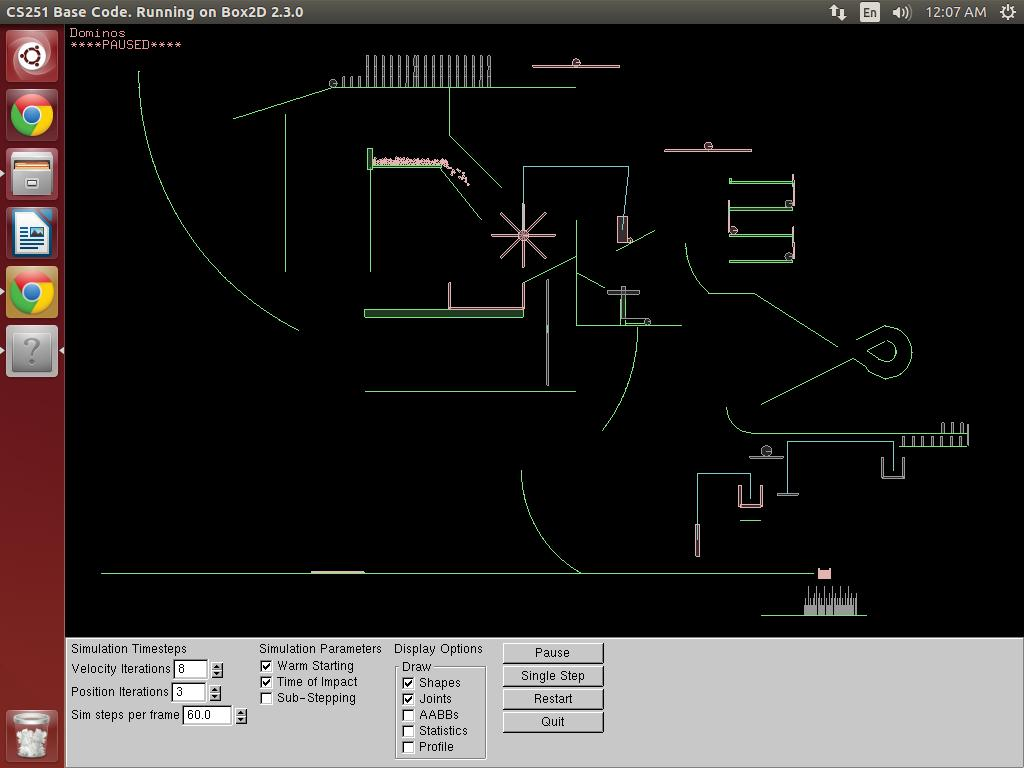
\includegraphics[scale=0.4]{FullProject}\\
\pagebreak

\section{List of components}
\begin{enumerate}
\item \textbf{The Dam} - The dam holds water and releases it as soon as the simulation begins. It also holds the water at the end of the simulation.\\\\
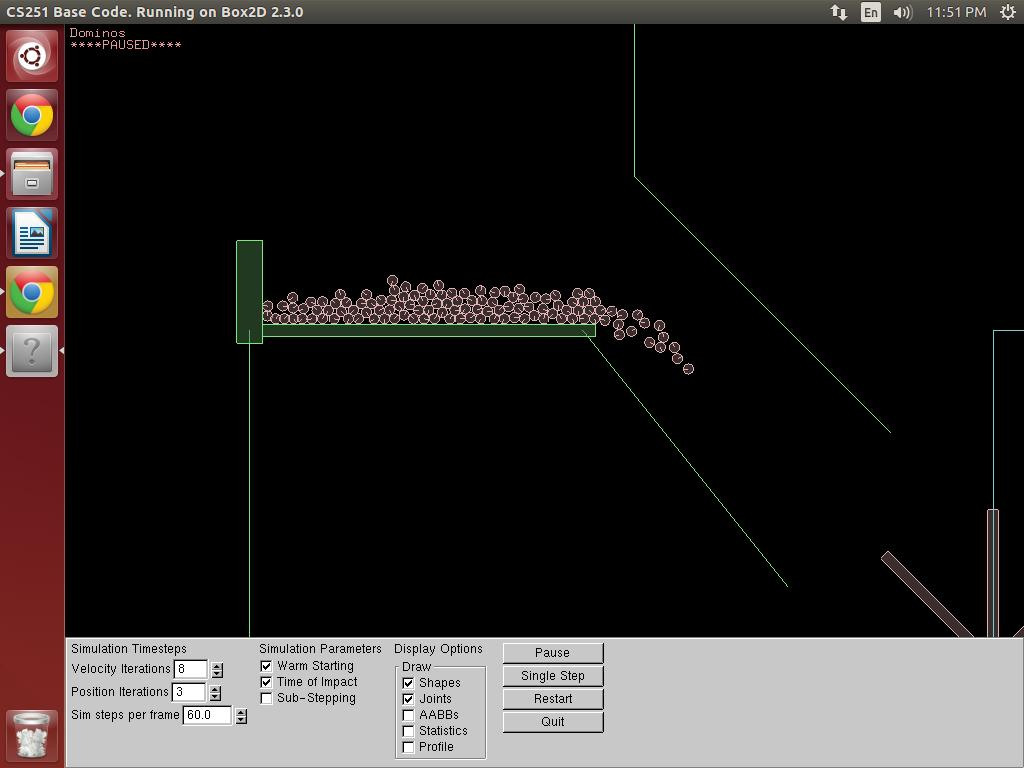
\includegraphics[scale=0.25]{pics/Dam}
\item \textbf{The Turbine} - The water released from the dam falls on the turbine and rotates it. This rotation pulls a rope which rotates the pulley thus activating a process on the other side of the pulley.\\\\
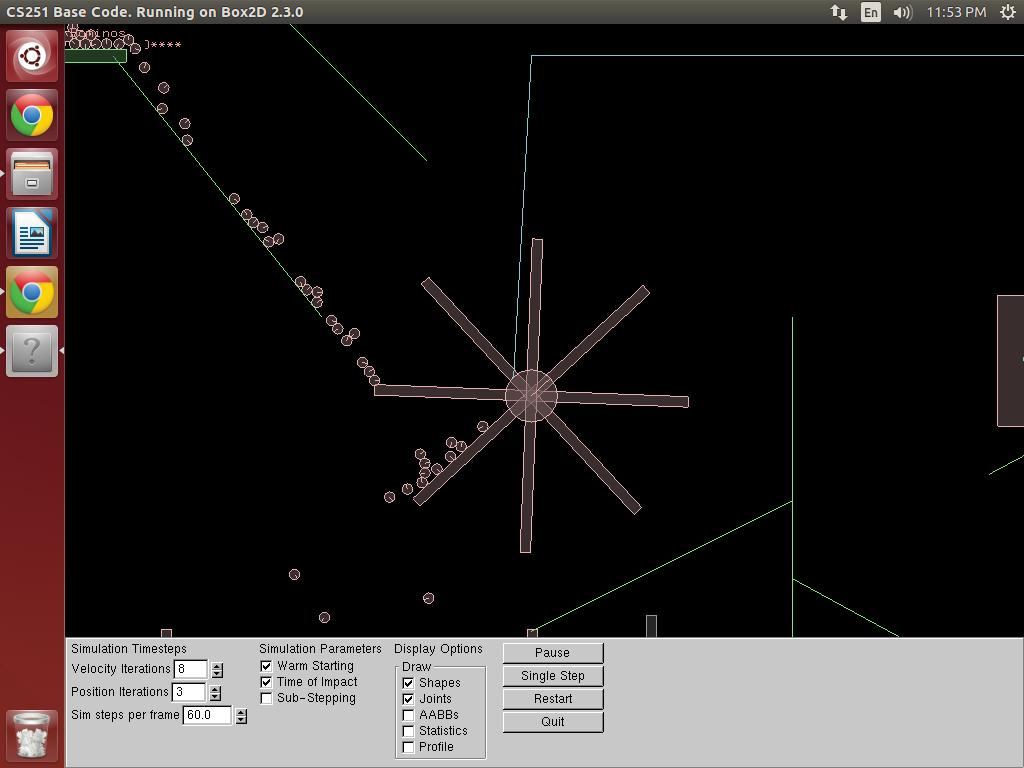
\includegraphics[scale=0.25]{pics/Turbine}\\
\pagebreak

\item \textbf{The Tub} - The tub collects the water after it has fallen on the turbine in order to feed it back to the dam.\\\\
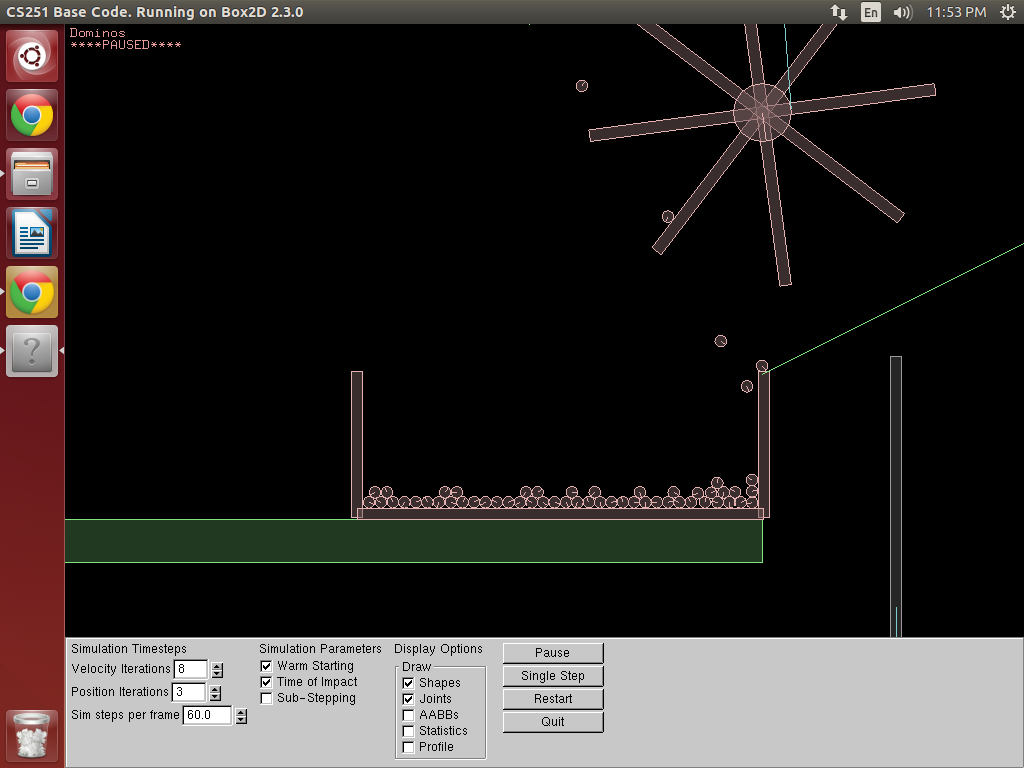
\includegraphics[scale=0.25]{pics/Tub}
\item \textbf{Pulley Joint} - When the turbine rotates, it uses the pulley joint to lift the bar at the other end. Once the bar lifts, it releases a ball blocked by it which then falls on the piston of the air-pump.\\\\
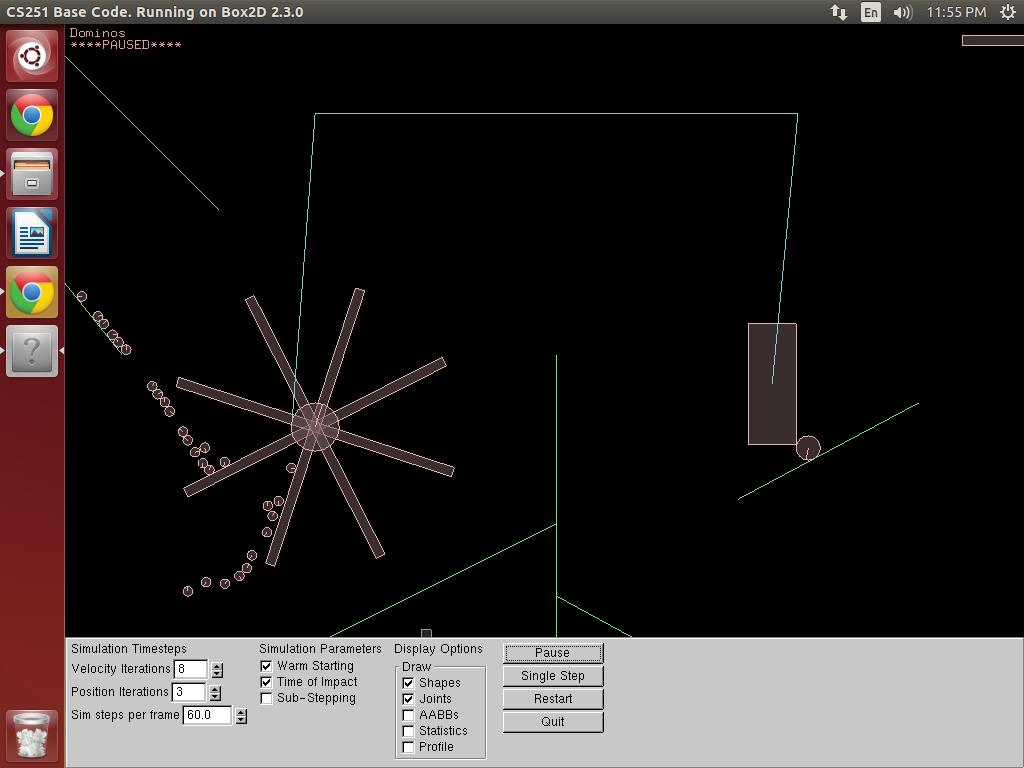
\includegraphics[scale=0.25]{pics/PulleyJointTurbineBox}
\pagebreak

\item \textbf{Air-pump} - When the ball falls on the piston of this pump, it releases a balloon trapped in it.\\\\
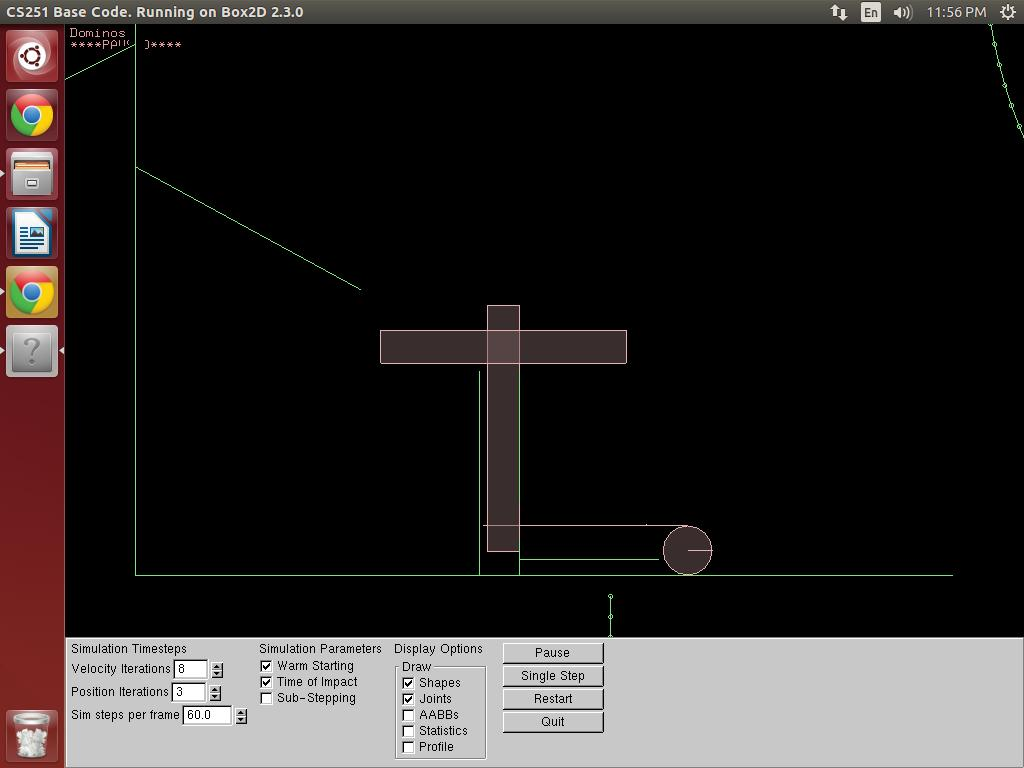
\includegraphics[scale=0.25]{pics/AirPump}
\item \textbf{Balloon} - The balloon is released by the Air-pump and it flies up to first hit a shaft to trigger further actions in the main simulation. After hitting this shaft, it further goes up to hit another shaft to trigger the water conservation model. When the shafts are hit they let a ball (which is initially carefully balanced on them) to fall and these balls further the simulation.\\\\
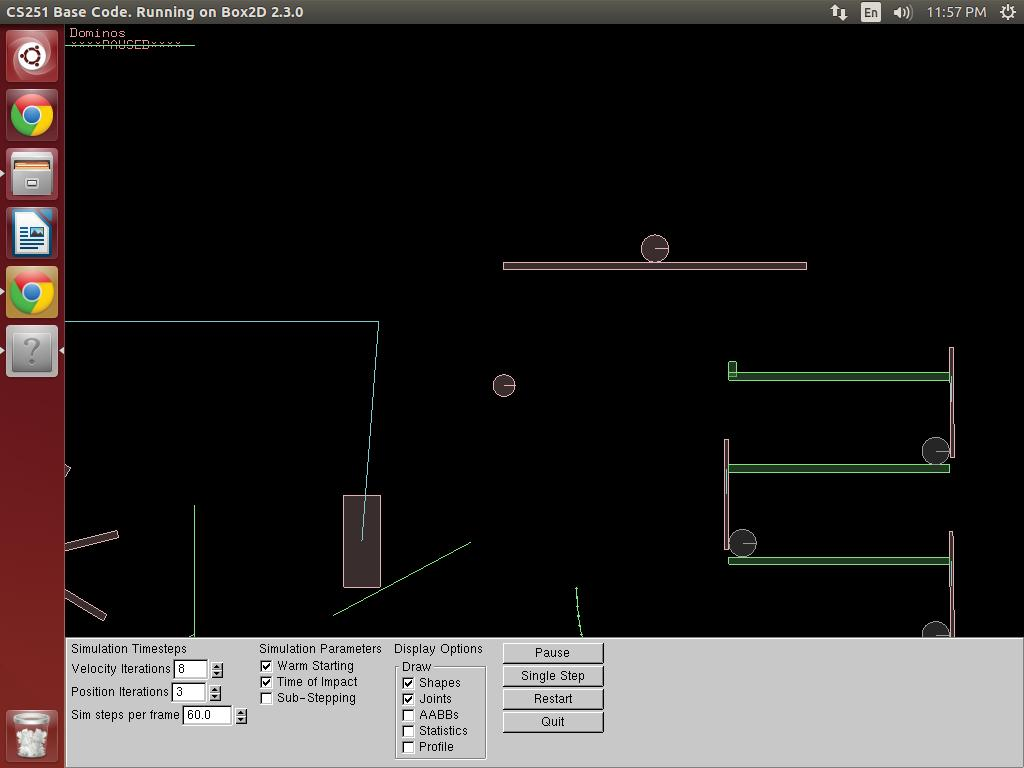
\includegraphics[scale=0.25]{pics/FlyingBalloon}
\pagebreak

\item \textbf{Ball-Hinge system} - Once the balloon hits the lower shaft and the ball balanced on it falls to the right and enters this ball-hinge system wherein the ball hits the first hinge which then hits another ball and this continues until the fourth ball is released onto a curved platform.\\\\
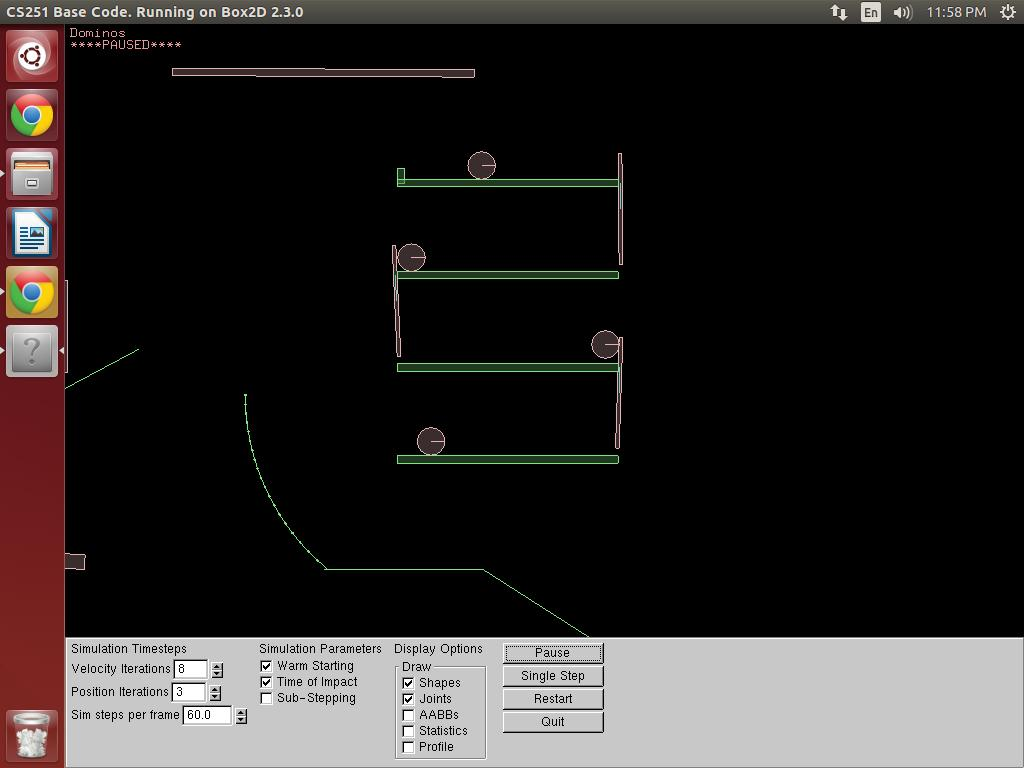
\includegraphics[scale=0.25]{pics/BallHingeSystem}
\item \textbf{Dominoes (Water conservation model)} - Once the balloon hits the higher shaft, the ball balanced on it falls to the left and hits this carefully balanced stack of dominoes. These dominoes then fall on one another and finally hit a heavy ball balanced on the left edge of this plank. This ball then falls to trigger further events in the water conservation model as well as the fire extinguisher model.\\\\
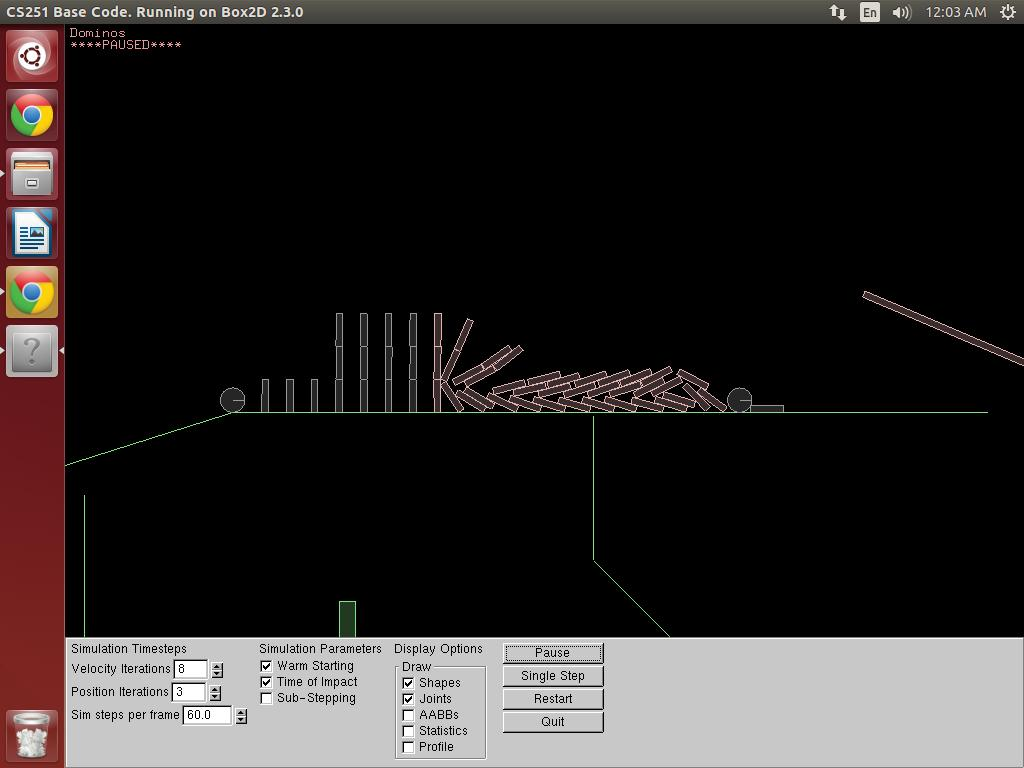
\includegraphics[scale=0.25]{pics/TopDominoMechanism}
\pagebreak

\item \textbf{Roller-Coaster} - The ball which releases from the Ball-hinge system passes through this roller-coaster and then falls into another plank and overturns a stack of dominoes after that.\\\\
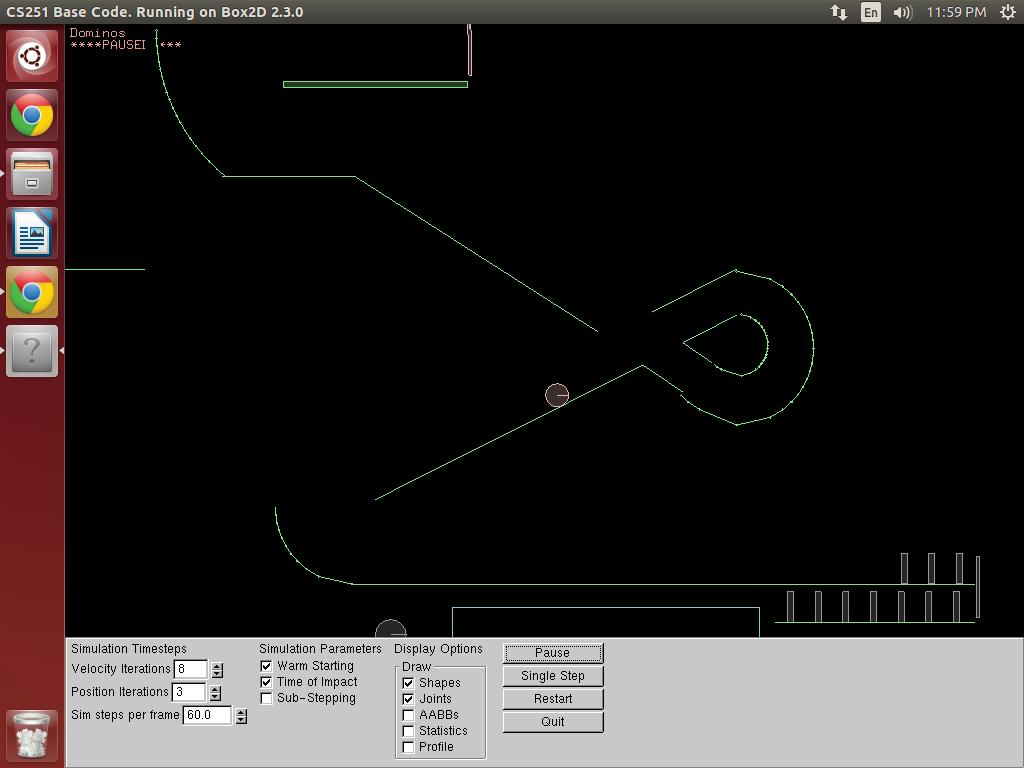
\includegraphics[scale=0.25]{pics/TunnelForBall}
\item \textbf{Revolving Plank (Water conservation model)} - The heavy ball hit by the stack of dominoes in the water conservation model falls and hits revolving plank directly underneath the water tub. On revolving, this plank pushes the tub towards the elevator which will lift it up to the dam. The heavy ball then further falls in order to spill a glass of water to extinguish fire in the bottom portion of the simulation.\\\\
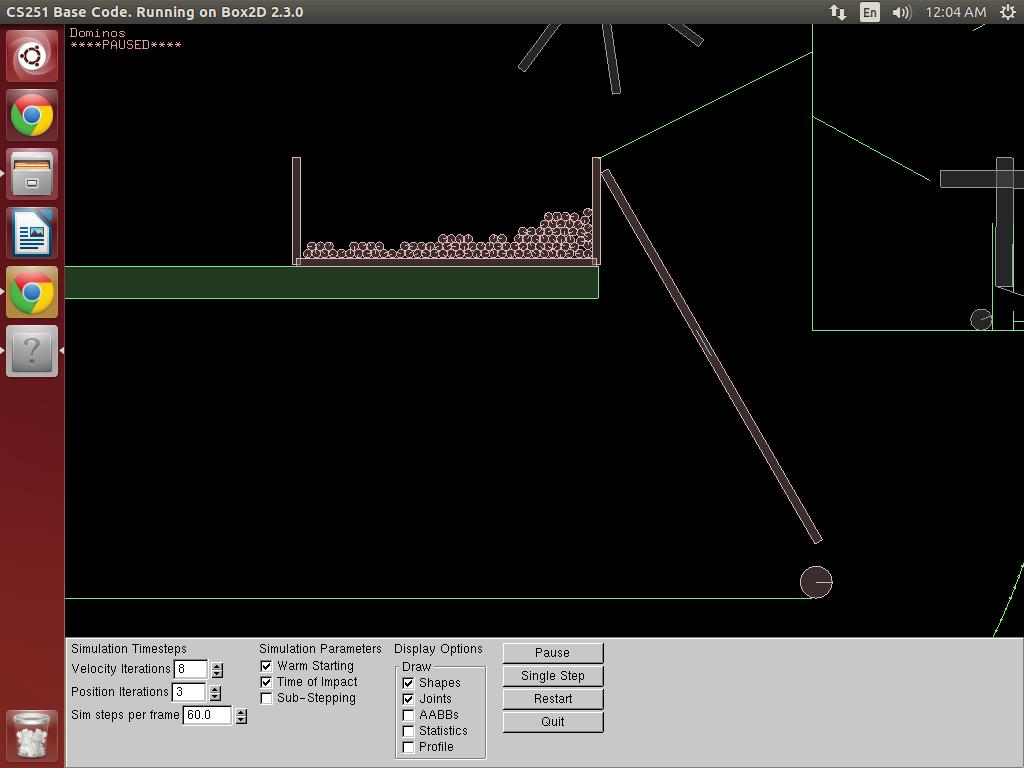
\includegraphics[scale=0.25]{pics/RevolvingPlankWaterBox}
\pagebreak

\item \textbf{Gate-Opening system} - Once the ball hits the stack of dominoes after passing through the roller coaster, this effect is carried forward by dominoes falling thorugh and the final domino then falls into a box connected to a pulley. This lifts the bar at the other end of the pulley which then hits a shaft and allows a carefully balanced ball to fall into another box connected to a pulley which has a gate connected to it. When this ball falls into this box, the gate raises due to the pulley joint to allow the heavy ball to pass through.\\
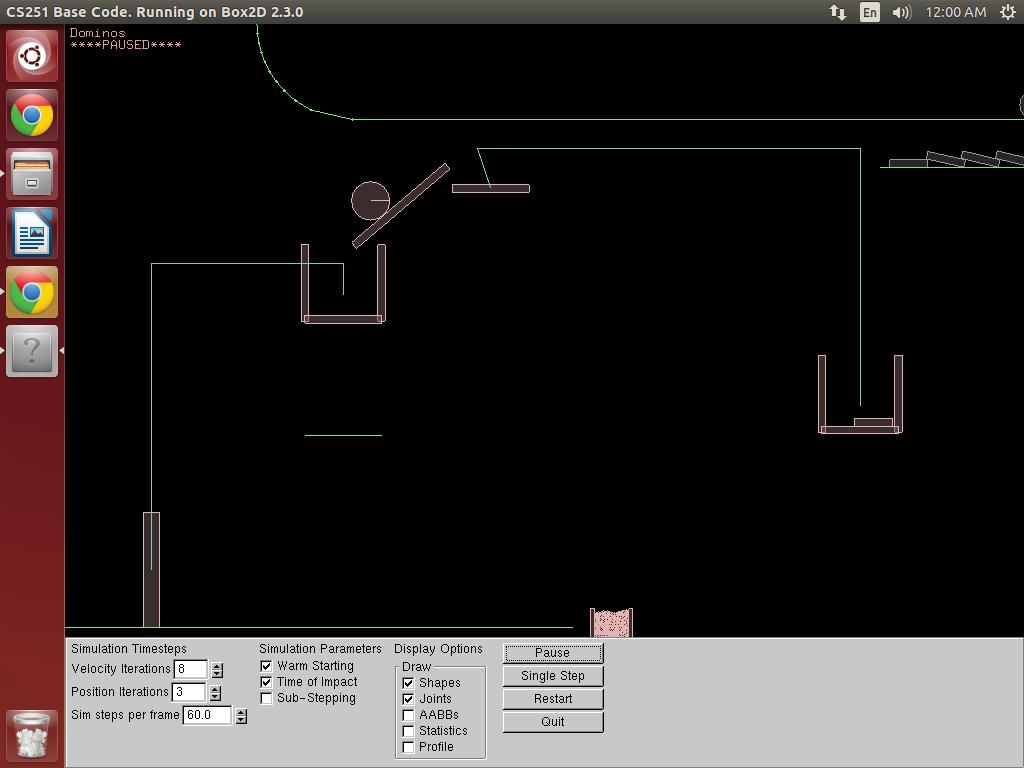
\includegraphics[scale=0.20]{pics/LowerGateMechanism}
\item \textbf{Curved platforms (Transition from the water conservation model to the main simulation)} - After rotating the plank in the water conservation model, the heavy ball falls through to a curved platform which leads to another curved platform. This platforms then drops it to the ground. Here, it is supposed to move and spill the glass of water onto the fire underneath but its advance is blocked by a gate. This gate is opened by the mechanism mentioned above just in time for this heavy ball to pass.\\
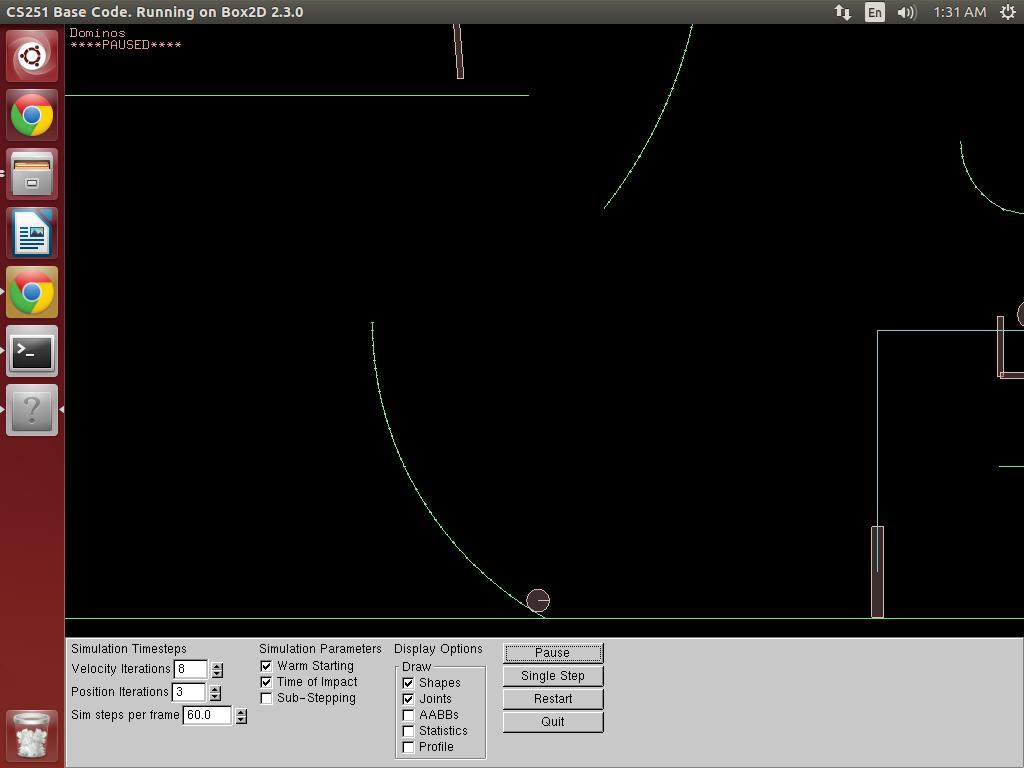
\includegraphics[scale=0.20]{pics/HeavyBall}
\pagebreak

\item \textbf{Fire} - The fire at the bottom-most part of the simulation region which is needed to be extinguished.\\\\
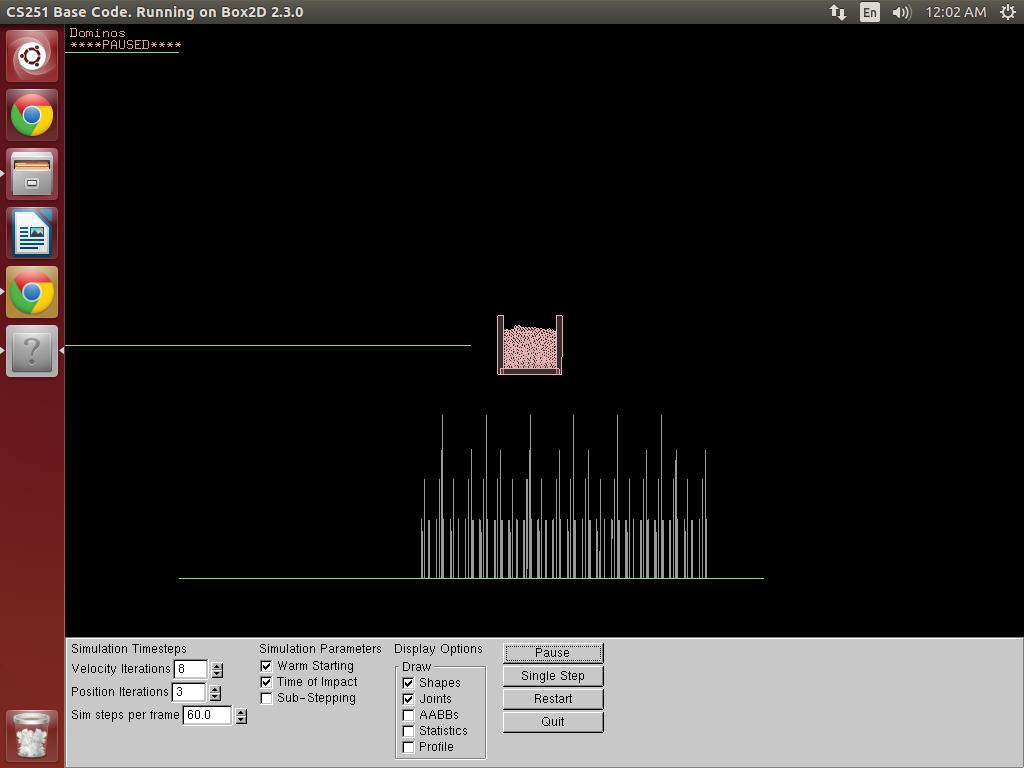
\includegraphics[scale=0.25]{pics/Fire}
\item \textbf{Elevator (Water conservation model)} - When the tub is hit by the revolving plank, it moves to the left and is caught by this slowly moving elevator shaft which lifts up the tub and puts the water back into the dam.\\\\
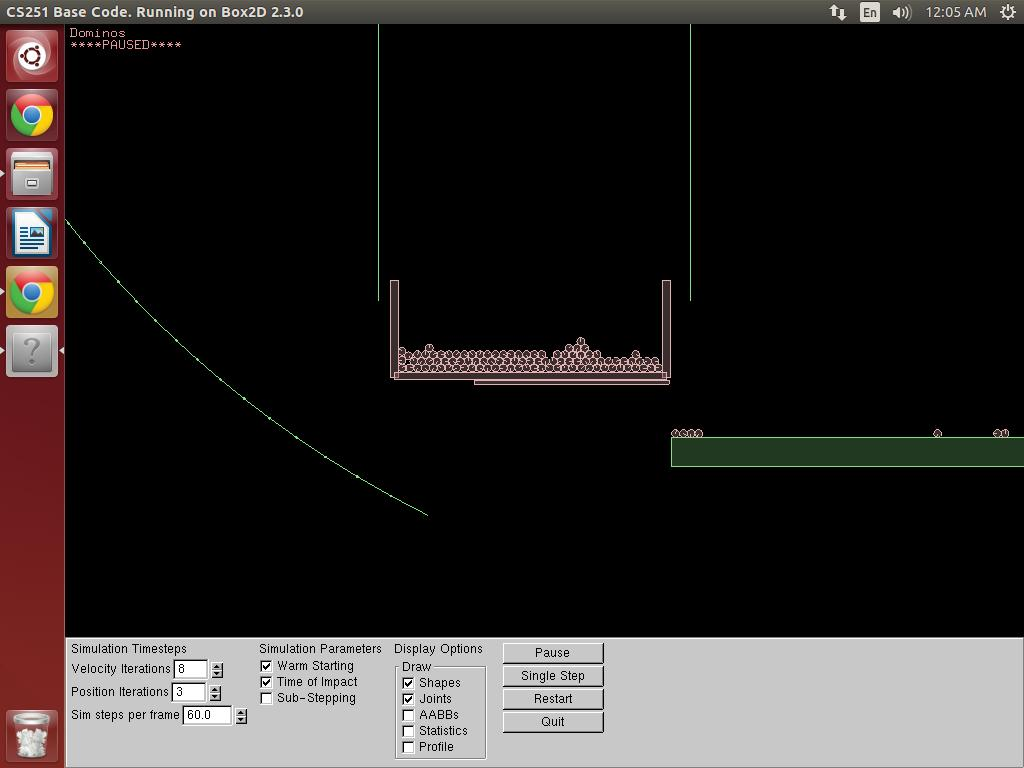
\includegraphics[scale=0.25]{pics/WaterBoxLift}
\pagebreak

\item \textbf{Water glass} - The last step of the simulation occurs when the heavy balls hits this glass of water which drops its contents into the fire underneath and extinguishes it.\\\\
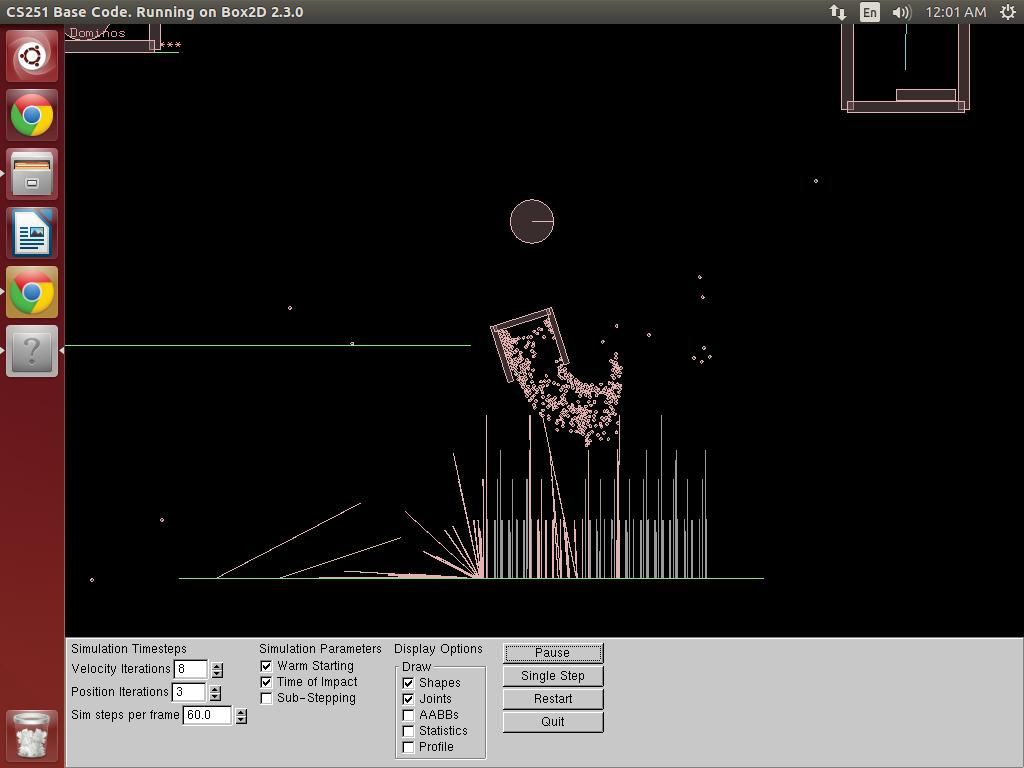
\includegraphics[scale=0.25]{pics/WaterGlassAndFire(extinguished)}

\end{enumerate}
\pagebreak

\chapter{Profiling and References}
\section{Profiling}
Earlier the functions consuming maximum time were:
\begin{enumerate}
\item b2ContactSolver::SolveVelocityConstraints()
\item b2Vec2::b2Vec2(float, float)
\item operator-(b2Vec2 const\&, b2Vec2 const\&)
\item operator+(b2Vec2 const\&, b2Vec2 const\&)
\item operator*(float, b2Vec2 const\&)
\end{enumerate}
Earlier the call graph image created was:\\

\includegraphics[scale=0.05]{performanceold}\\

Now the functions consuming maximum time are:
\begin{enumerate}
\item b2ContactSolver::SolveVelocityConstraints()
\item operator-(b2Vec2 const\&, b2Vec2 const\&)
\item operator*(float, b2Vec2 const\&)
\item b2Vec2::b2Vec2(float, float)
\item b2World::SolveTOI(b2TimeStep const\&)
\end{enumerate}

Now the call graph image created is:\\

\includegraphics[scale=0.05]{performancenew}\\

\section{Concepts learnt and used}
\begin{itemize}
\item Using a physics engine - \textbf{Box2D}.
\item Preparing documentation - \textbf{Doxygen}.
\item Preparing a report and a presentation - \textbf{Latex}.
\item Profiling our code - \textbf{gprof}.
\item Preparing a webpage for the project - \textbf{HTML, CSS and Javascript}.
\item Version control - \textbf{git}.
\item Preparing makefiles to run the code - \textbf{Makefile}
\end{itemize}

\section{Honour Code}
We pledge on our honour as students that : 
\begin{enumerate}
\item We haven't taken/given inputs from/to other groups.
\item We have reported our contributions to the assignment accurately to the best of our knowledge.
\end{enumerate}

\section{Individual Contribution}
\begin{itemize}
\item 140040005 - 100\% 
\item 14D070027 - 100\% 
\item 14D070063 - 100\% 
\end{itemize}

%\printbibliography
\section{References}
\begin{enumerate}
 \item CS251-Software Systems Lab\\
    Outlab3 - cs251\_box2d\_base as the base code for the project\\
    http://www.cse.iitb.ac.in/~sharat/current/cs251/Assign/Lab03/
 \item CS251-Software Systems Lab\\
    Outlab9 - cs251\_box2d\_base with doxyfile and modified makefile taken from here\\
    http://www.cse.iitb.ac.in/~sharat/current/cs251/Assign/Lab03/
 \item Box2D manual (From the site- www.box2d.org)\\
    http://box2d.org/manual.pdf
 \item Box2D C++ Tutorials (From the site- www.iforce2d.net)\\
    http://www.iforce2d.net/b2dtut/
 \item Box2D Forums (From the site- www.box2d.org) \\
    http://box2d.org/forum/viewtopic.php?f=19\&t=9079
 \item ChainShape (libgdx API) \\
    https://libgdx.badlogicgames.com/nightlies/docs/api/com/badlogic/gdx/physics/box2d/ChainShape.html
 \item Box2D Tutorials\\
    http://www.iforce2d.net/b2dtut/custom-gravity
 \item GPROF Tutorial\\
    http://www.thegeekstuff.com/2012/08/gprof-tutorial/
 \item Doxygen Manual\\
    http://www.stack.nl/~dimitri/doxygen/manual/index.html
 \item LaTeX Documentation\\
     http://texdoc.net/texmf-dist/doc/latex/latex2e-help-texinfo/latex2e.pdf
 \item BibTeX Example\\
     https://verbosus.com/bibtex-style-examples.html
 \item MakeFile Tutorial\\
     http://www.tutorialspoint.com/makefile/
\end{enumerate}

\end{document}
